% GNUPLOT: LaTeX picture with Postscript
\begingroup
  \makeatletter
  \providecommand\color[2][]{%
    \GenericError{(gnuplot) \space\space\space\@spaces}{%
      Package color not loaded in conjunction with
      terminal option `colourtext'%
    }{See the gnuplot documentation for explanation.%
    }{Either use 'blacktext' in gnuplot or load the package
      color.sty in LaTeX.}%
    \renewcommand\color[2][]{}%
  }%
  \providecommand\includegraphics[2][]{%
    \GenericError{(gnuplot) \space\space\space\@spaces}{%
      Package graphicx or graphics not loaded%
    }{See the gnuplot documentation for explanation.%
    }{The gnuplot epslatex terminal needs graphicx.sty or graphics.sty.}%
    \renewcommand\includegraphics[2][]{}%
  }%
  \providecommand\rotatebox[2]{#2}%
  \@ifundefined{ifGPcolor}{%
    \newif\ifGPcolor
    \GPcolorfalse
  }{}%
  \@ifundefined{ifGPblacktext}{%
    \newif\ifGPblacktext
    \GPblacktexttrue
  }{}%
  % define a \g@addto@macro without @ in the name:
  \let\gplgaddtomacro\g@addto@macro
  % define empty templates for all commands taking text:
  \gdef\gplbacktext{}%
  \gdef\gplfronttext{}%
  \makeatother
  \ifGPblacktext
    % no textcolor at all
    \def\colorrgb#1{}%
    \def\colorgray#1{}%
  \else
    % gray or color?
    \ifGPcolor
      \def\colorrgb#1{\color[rgb]{#1}}%
      \def\colorgray#1{\color[gray]{#1}}%
      \expandafter\def\csname LTw\endcsname{\color{white}}%
      \expandafter\def\csname LTb\endcsname{\color{black}}%
      \expandafter\def\csname LTa\endcsname{\color{black}}%
      \expandafter\def\csname LT0\endcsname{\color[rgb]{1,0,0}}%
      \expandafter\def\csname LT1\endcsname{\color[rgb]{0,1,0}}%
      \expandafter\def\csname LT2\endcsname{\color[rgb]{0,0,1}}%
      \expandafter\def\csname LT3\endcsname{\color[rgb]{1,0,1}}%
      \expandafter\def\csname LT4\endcsname{\color[rgb]{0,1,1}}%
      \expandafter\def\csname LT5\endcsname{\color[rgb]{1,1,0}}%
      \expandafter\def\csname LT6\endcsname{\color[rgb]{0,0,0}}%
      \expandafter\def\csname LT7\endcsname{\color[rgb]{1,0.3,0}}%
      \expandafter\def\csname LT8\endcsname{\color[rgb]{0.5,0.5,0.5}}%
    \else
      % gray
      \def\colorrgb#1{\color{black}}%
      \def\colorgray#1{\color[gray]{#1}}%
      \expandafter\def\csname LTw\endcsname{\color{white}}%
      \expandafter\def\csname LTb\endcsname{\color{black}}%
      \expandafter\def\csname LTa\endcsname{\color{black}}%
      \expandafter\def\csname LT0\endcsname{\color{black}}%
      \expandafter\def\csname LT1\endcsname{\color{black}}%
      \expandafter\def\csname LT2\endcsname{\color{black}}%
      \expandafter\def\csname LT3\endcsname{\color{black}}%
      \expandafter\def\csname LT4\endcsname{\color{black}}%
      \expandafter\def\csname LT5\endcsname{\color{black}}%
      \expandafter\def\csname LT6\endcsname{\color{black}}%
      \expandafter\def\csname LT7\endcsname{\color{black}}%
      \expandafter\def\csname LT8\endcsname{\color{black}}%
    \fi
  \fi
    \setlength{\unitlength}{0.0500bp}%
    \ifx\gptboxheight\undefined%
      \newlength{\gptboxheight}%
      \newlength{\gptboxwidth}%
      \newsavebox{\gptboxtext}%
    \fi%
    \setlength{\fboxrule}{0.5pt}%
    \setlength{\fboxsep}{1pt}%
\begin{picture}(5668.00,3400.00)%
    \gplgaddtomacro\gplbacktext{%
      \csname LTb\endcsname%%
      \put(434,2717){\makebox(0,0)[r]{\strut{}$0$}}%
      \csname LTb\endcsname%%
      \put(434,3009){\makebox(0,0)[r]{\strut{}$0.9$}}%
      \csname LTb\endcsname%%
      \put(434,3300){\makebox(0,0)[r]{\strut{}$1.8$}}%
      \csname LTb\endcsname%%
      \put(566,2432){\makebox(0,0){\strut{}}}%
      \csname LTb\endcsname%%
      \put(1369,2432){\makebox(0,0){\strut{}}}%
      \csname LTb\endcsname%%
      \put(2172,2432){\makebox(0,0){\strut{}}}%
      \csname LTb\endcsname%%
      \put(2975,2432){\makebox(0,0){\strut{}}}%
      \csname LTb\endcsname%%
      \put(3777,2432){\makebox(0,0){\strut{}}}%
      \csname LTb\endcsname%%
      \put(4580,2432){\makebox(0,0){\strut{}}}%
      \csname LTb\endcsname%%
      \put(5383,2432){\makebox(0,0){\strut{}}}%
    }%
    \gplgaddtomacro\gplfronttext{%
      \csname LTb\endcsname%%
      \put(-171,3008){\rotatebox{-270}{\makebox(0,0){\strut{}$Q$}}}%
      \put(2974,2366){\makebox(0,0){\strut{}}}%
    }%
    \gplgaddtomacro\gplbacktext{%
      \csname LTb\endcsname%%
      \put(434,2002){\makebox(0,0)[r]{\strut{}$0$}}%
      \csname LTb\endcsname%%
      \put(434,2294){\makebox(0,0)[r]{\strut{}$0.9$}}%
      \csname LTb\endcsname%%
      \put(434,2586){\makebox(0,0)[r]{\strut{}$1.8$}}%
      \csname LTb\endcsname%%
      \put(566,1717){\makebox(0,0){\strut{}}}%
      \csname LTb\endcsname%%
      \put(1369,1717){\makebox(0,0){\strut{}}}%
      \csname LTb\endcsname%%
      \put(2172,1717){\makebox(0,0){\strut{}}}%
      \csname LTb\endcsname%%
      \put(2975,1717){\makebox(0,0){\strut{}}}%
      \csname LTb\endcsname%%
      \put(3777,1717){\makebox(0,0){\strut{}}}%
      \csname LTb\endcsname%%
      \put(4580,1717){\makebox(0,0){\strut{}}}%
      \csname LTb\endcsname%%
      \put(5383,1717){\makebox(0,0){\strut{}}}%
    }%
    \gplgaddtomacro\gplfronttext{%
      \csname LTb\endcsname%%
      \put(-171,2294){\rotatebox{-270}{\makebox(0,0){\strut{}$CLK$}}}%
      \put(2974,1651){\makebox(0,0){\strut{}}}%
    }%
    \gplgaddtomacro\gplbacktext{%
      \csname LTb\endcsname%%
      \put(434,1289){\makebox(0,0)[r]{\strut{}$0$}}%
      \csname LTb\endcsname%%
      \put(434,1581){\makebox(0,0)[r]{\strut{}$0.9$}}%
      \csname LTb\endcsname%%
      \put(434,1872){\makebox(0,0)[r]{\strut{}$1.8$}}%
      \csname LTb\endcsname%%
      \put(566,1004){\makebox(0,0){\strut{}}}%
      \csname LTb\endcsname%%
      \put(1369,1004){\makebox(0,0){\strut{}}}%
      \csname LTb\endcsname%%
      \put(2172,1004){\makebox(0,0){\strut{}}}%
      \csname LTb\endcsname%%
      \put(2975,1004){\makebox(0,0){\strut{}}}%
      \csname LTb\endcsname%%
      \put(3777,1004){\makebox(0,0){\strut{}}}%
      \csname LTb\endcsname%%
      \put(4580,1004){\makebox(0,0){\strut{}}}%
      \csname LTb\endcsname%%
      \put(5383,1004){\makebox(0,0){\strut{}}}%
    }%
    \gplgaddtomacro\gplfronttext{%
      \csname LTb\endcsname%%
      \put(-171,1580){\rotatebox{-270}{\makebox(0,0){\strut{}$S$}}}%
      \put(2974,938){\makebox(0,0){\strut{}}}%
    }%
    \gplgaddtomacro\gplbacktext{%
      \csname LTb\endcsname%%
      \put(434,575){\makebox(0,0)[r]{\strut{}$0$}}%
      \csname LTb\endcsname%%
      \put(434,867){\makebox(0,0)[r]{\strut{}$0.9$}}%
      \csname LTb\endcsname%%
      \put(434,1158){\makebox(0,0)[r]{\strut{}$1.8$}}%
      \csname LTb\endcsname%%
      \put(566,290){\makebox(0,0){\strut{}0}}%
      \csname LTb\endcsname%%
      \put(1369,290){\makebox(0,0){\strut{}60}}%
      \csname LTb\endcsname%%
      \put(2172,290){\makebox(0,0){\strut{}120}}%
      \csname LTb\endcsname%%
      \put(2975,290){\makebox(0,0){\strut{}180}}%
      \csname LTb\endcsname%%
      \put(3777,290){\makebox(0,0){\strut{}240}}%
      \csname LTb\endcsname%%
      \put(4580,290){\makebox(0,0){\strut{}300}}%
      \csname LTb\endcsname%%
      \put(5383,290){\makebox(0,0){\strut{}360}}%
    }%
    \gplgaddtomacro\gplfronttext{%
      \csname LTb\endcsname%%
      \put(-171,866){\rotatebox{-270}{\makebox(0,0){\strut{}$R$}}}%
      \put(2974,-40){\makebox(0,0){\strut{}tempo $[ns]$}}%
    }%
    \gplbacktext
    \put(0,0){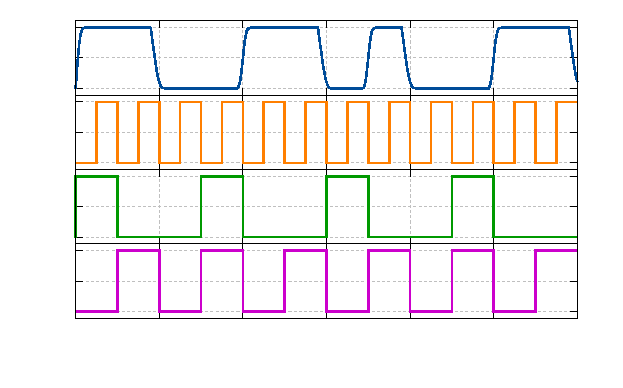
\includegraphics[width={283.40bp},height={170.00bp}]{Immagini/jkff-ms-sim}}%
    \gplfronttext
  \end{picture}%
\endgroup

